\documentclass{article}
\usepackage[utf8]{inputenc}
\usepackage{amsfonts}
\usepackage{mathtools}
\usepackage{tikz}
\usepackage{caption}
\usepackage{subcaption}
\usepackage{hyperref}
\usepackage{geometry}
\usepackage{amsthm}
\theoremstyle{remark}
\newtheorem*{remark}{Remark}
\geometry{a4paper}
\newcommand{\T}{\mathsf{T}}
\newcommand{\V}{\mathsf{V}}
\newcommand{\K}{\mathsf{K}}
\newcommand{\W}{\mathsf{W}}
\newcommand{\Id}{\mathsf{Id}}
\newcommand{\aaa}{\mathsf{a}}
\newcommand{\bbb}{\mathsf{b}}
\newcommand{\hata}{\widehat{\aaa}}
\newcommand{\hatb}{\widehat{\bbb}}
\newcommand{\hatell}{\widehat{\ell}}
\newcommand{\x}{\boldsymbol{x}}
\newcommand{\y}{\boldsymbol{y}}
\newcommand{\dd}{\mathrm{d}}
\newcommand{\n}{\boldsymbol{n}}
\newcommand{\tg}{\boldsymbol{t}}
\newcommand{\hatx}{\widehat{\boldsymbol{x}}}
\newcommand{\haty}{\widehat{\boldsymbol{y}}}
\newcommand{\argu}{\mathfrak{u}}
\newcommand{\argv}{\mathfrak{v}}
\newcommand{\argf}{\mathfrak{f}}
\newcommand{\argg}{\mathfrak{g}}
\newcommand{\tildeg}{\widetilde{\argg}}
\newcommand{\hatu}{\widehat{\argu}}
\newcommand{\hatv}{\widehat{\argv}}
\newcommand{\hatf}{\widehat{\argf}}
\newcommand{\hatpsi}{\widehat{\psi}}
\newcommand{\hatphi}{\widehat{\phi}}
\newcommand{\hatvphi}{\widehat{\varphi}}
\newcommand{\vv}[1]{\vec{\boldsymbol{#1}}}
\newcommand{\mat}[1]{\mathbf{#1}}
\newcommand{\Eps}{\mathcal{E}}
\newcommand{\hatEps}{\widehat{\Eps}}
\newcommand{\hatJ}{\widehat{J}}
\newcommand{\Nu}{\mathcal{V}}
\newcommand{\DNu}{\mathsf{D}\Nu}
\newcommand{\Tt}{\T_\Nu^t}
\newcommand{\DTt}{\mathsf{DT}_\Nu^t}
\newcommand{\CDTt}[1]{\mat{C}(\DTt({#1}))}
\newcommand{\ot}{\omega_t}
\newcommand{\hatfuncf}{\widehat{f}}

\title{Term Project\\\textbf{BEM-Based Computation of Forces on Dielectrics}}
\author{Ning Ren\\[1ex]Supervisors: Prof. Dr. Ralf Hiptmair, Piyush Panchal}
\date{February 2022}

\begin{document}

\maketitle
\tableofcontents

\newpage

\section{Introduction}
\subsection{Model Problem}
A parallel-plate capacitor is filled with two homogeneous isotropic linear dielectric materials. Dielectric $i$ of permittivity $\varepsilon_i$ fills the bounded open connected Lipschitz domain $\Omega_i\subset\mathbb{R}^2$ where $i=1,2$. Dielectric $1$ is embedded in dielectric $2$. A potential difference $U$ is imposed between the plates of the capacitor. We use short notations $\Omega\coloneqq\Omega_1\cup\Omega_2\subset\mathbb{R}^2$ for the field domain, $\Gamma_I\coloneqq\partial\Omega_1$ for the interface between two dielectrics, $\Gamma_D\subset\partial\Omega$ for the edges of dielectric $2$ touching the capacitor and $\Gamma_N\coloneqq\partial\Omega\setminus\Gamma_D$.

Writing $\n$ for the exterior unit normal vector field on $\partial\Omega_2$, the electrostatic scalar potential $u:\Omega\to\mathbb{R}$ is a weak solution in $H^1(\Omega)$ of the linear elliptic boundary value problem
\begin{equation}
\label{eq:bvp}
    \Delta u =0\quad\text{in}\quad\Omega,\quad u=\argg\quad\text{on}\quad\Gamma_D,\quad\nabla u\cdot\n=\eta\quad\text{on}\quad\Gamma_N
\end{equation}
Restricting $u$ to subdomains as $u_1\coloneqq \left.u\right|_{\Omega_1}, u_2\coloneqq \left.u\right|_{\Omega_2}$, the transmission conditions of this problem are
\begin{equation}
\label{eq:trans-cond}
    \left.u_1\right|_{\Gamma_I} = \left.u_2\right|_{\Gamma_I},\quad\varepsilon_1\left.\nabla u_1\cdot\n_1\right|_{\Gamma_I}=-\varepsilon_2\left.\nabla u_2\cdot\n_2\right|_{\Gamma_I},
\end{equation}
where $\n_1\coloneqq-\n,~\n_2\coloneqq\n$ on $\Gamma_I$.

\begin{figure}[h]
    \centering
    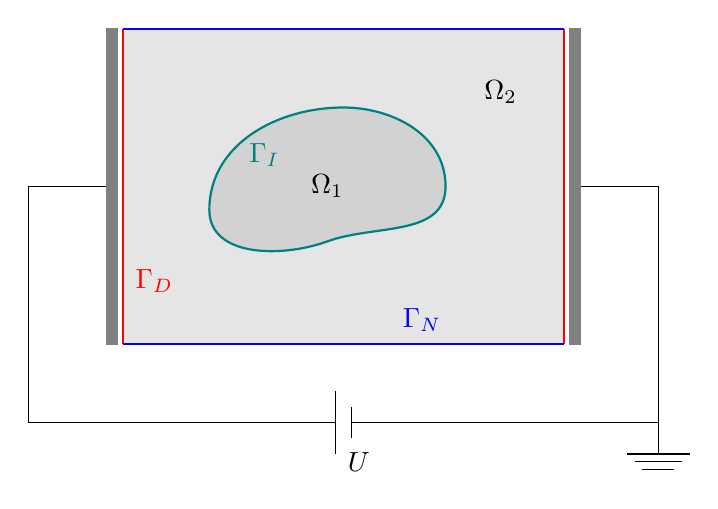
\begin{tikzpicture}
    \draw (1,4)--(0,4)--(0,1)--(3.9,1); % left wire
    \draw (4.1,1)--(8,1); \draw (8,0.6)--(8,4)--(7,4); % right wire
    \draw (3.9,0.6)--(3.9,1.4); \draw (4.1,0.8)--(4.1,1.2); % battery
    \draw (7.6,0.6)--(8.4,0.6); \draw (7.7,0.5)--(8.3,0.5); \draw (7.8,0.4)--(8.2,0.4); % earthing
    \draw [gray,thick,fill=gray] (1,2) rectangle (1.12,6); % left plate
    \draw [gray,thick,fill=gray] (6.88,2) rectangle (7,6); % right plate
    \path [fill=white!50!gray!40] (1.2,2) rectangle (6.8,6); % outer
    \draw [red,thick] (1.2,2)--(1.2,6); \draw [red,thick] (6.8,2)--(6.8,6); % Gamma_D
    \draw [blue,thick] (1.2,2)--(6.8,2); \draw [blue,thick] (1.2,6)--(6.8,6); % Gamma_N
    \draw [teal,thick,fill=white!30!gray!50] (2.3,3.7) to [out=90,in=180] (4,5) to [out=0,in=90] (5.3,4) to [out=270,in=20] (3.8,3.3) to [out=200,in=270] (2.3,3.7); % inner
    
    \node at (4.2,0.5) {$U$};
    \node at (3.8,4) {$\Omega_1$};
    \node at (6,5.2) {$\Omega_2$};
    \node [teal] at (3,4.4) {$\Gamma_I$};
    \node [red] at (1.6,2.8) {$\Gamma_D$};
    \node [blue] at (5,2.3) {$\Gamma_N$};
    \end{tikzpicture}
    \caption{Geometric setting for model problem}
    \label{fig:model}
\end{figure}
Figure~\ref{fig:model} shows a specific physical setting. On $\Gamma_D$, the Dirichlet data is constant on each plate with $\argg\equiv U$ on the left plate and $\argg\equiv 0$ on the right plate. The fringing field around the edges is ignored, and therefore the Neumann data $\eta\equiv 0$ on $\Gamma_N$\cite[Section~4.4]{griffiths_2017}. Nevertheless, general $\argg\in H^{\frac{1}{2}}(\Gamma_D)$ and $\eta\in H^{-\frac{1}{2}}(\Gamma_N)$ are admitted.

\subsection{Classical Formulae for Forces}
For a linear dielectric of permittivity $\varepsilon$ in a static electric field, the Maxwell stress tensor \cite[Section~8.2]{griffiths_2017} is defined as
\begin{equation}
    \mat{T}(u)\coloneqq\varepsilon\left(\nabla u\nabla u^\top - \frac{1}{2}\|\nabla u\|^2\mat{I}_d\right)
\end{equation}
with the electrostatic potential $u$. At material interfaces, the Maxwell stress tensor is generally discontinuous and the surface force density $\mat{f}^{\Gamma}$ is defined as the jump of
$\mat{T}(u)\cdot\n$~\cite{force}. The total force on the dielectric $1$ is given by
\begin{equation}
\label{eq:force}
    \mat{F}\coloneqq\int_{\Gamma_I}\mat{f}^\Gamma\,\dd S
    =\int_{\Gamma_I}\left(\mat{T}(u_2)-\mat{T}(u_1)\right)\n\,\dd S.
\end{equation}
Since $\Delta u=0$, we have $\nabla\cdot\mat{T}=0$. With permittivity
\begin{equation}
    \varepsilon(\x)\coloneqq
    \begin{cases}
		\varepsilon_1\quad\text{if}~\x\in\Omega_1,\\
        \varepsilon_2\quad\text{if}~\x\in\Omega_2,
	\end{cases}
\end{equation}
the divergence theorem yields the volume-based formula
\begin{equation}
\label{eq:vol-formula}
\begin{aligned}
    \mat{F}&=\int_{\Gamma_I}\mat{T}(u_1)\n_1\,w\,\dd S+\int_{\Gamma_I}\mat{T}(u_2)\n_2\,w\,\dd S+\int_{\partial\Omega}\mat{T}(u_2)\n_2\,w\,\dd S\\
    &=\int_{\Omega_1}\mat{T}(u_1)\nabla w\,\dd\x+\int_{\Omega_2}\mat{T}(u_2)\nabla w\,\dd\x\\
    &=\int_{\Omega}\varepsilon\left(\nabla u\left(\nabla u\cdot\nabla w\right)-\frac{1}{2}\|\nabla u\|^2\,\nabla w\right)\dd\x
\end{aligned}
\end{equation}
for any $\left.w\right|_{\Gamma_I}\equiv 1$ and $\left.w\right|_{\partial\Omega}\equiv 0$.

\section{Boundary Element Method (BEM)}
\subsection{Boundary Integral Equations (BIEs)}
For the transmission problem (\ref{eq:bvp}), the solution $u$ can be recovered from the traces on $\partial\Omega_2$. With boundary data extended to all of $\partial\Omega$
\begin{equation}
\begin{aligned}
    \argg'&\in H^{\frac{1}{2}}(\partial\Omega):&\quad\argg'|_{\Gamma_D}&=\argg,\\
    \eta'&\in H^{-\frac{1}{2}}(\partial\Omega):&\quad\eta'|_{\Gamma_N}&=\eta,
\end{aligned}
\end{equation}
we can seek the unknown traces on $\partial\Omega$ using the offset function technique
\begin{equation}
\begin{aligned}
    \left.u\right|_{\partial\Omega}&=\argg'+\argu,&&\argu\in H^{\frac{1}{2}}_{\Gamma_D}(\partial\Omega)\coloneqq\{\argv\in H^{\frac{1}{2}}:\left.\argv\right|_{\Gamma_D}=0\},\\
    \left.u\cdot\n\right|_{\partial\Omega}&=\eta'+\psi,&&\psi\in H^{-\frac{1}{2}}_{\Gamma_N}(\partial\Omega)\coloneqq\{\phi\in H^{-\frac{1}{2}}:\left.\phi\right|_{\Gamma_N}=0\}.
\end{aligned}
\end{equation}
Traces on $\Gamma_I$ are denoted as
$\argu_I\coloneqq\left.u\right|_{\Gamma_I}$ and $\psi_I\coloneqq\left.\nabla u_2\cdot\n\right|_{\Gamma_I}$. Using transmission conditions (\ref{eq:trans-cond}), the boundary data and the unknowns lead to the variational boundary integral equations:
\begin{equation*}
    \text{seek}~\argu_I\in H^{\frac{1}{2}}(\Gamma_I),
    ~\psi_I\in H^{-\frac{1}{2}}(\Gamma_I),
    ~\argu\in H^{\frac{1}{2}}_{\Gamma_D}(\partial\Omega),
    ~\psi\in H^{-\frac{1}{2}}_{\Gamma_N}(\partial\Omega):
\end{equation*}
\begin{multline*}
    \left(\frac{\varepsilon_1}{\varepsilon_2}+1\right)\aaa_{W,II}(\argu_I,\argv_I)+2\aaa_{K,II}(\argv_I,\psi_I)+\aaa_{W,NI}(\argu,\argv_I)+\aaa_{K,ID}(\argv_I,\psi)\\
    =-\bbb_{W,DI}(\argg,\argv_I)-\bbb_{K,IN}(\argv_I,\eta)\quad
    \forall\argv_I\in H^{\frac{1}{2}}(\Gamma_I),
\end{multline*}
\begin{multline*}
    2\,\aaa_{K,II}(\argu_I,\phi_I)-\left(\frac{\varepsilon_2}{\varepsilon_1}+1\right)\aaa_{V,II}(\psi_I,\phi_I)+\aaa_{K,NI}(\argu,\phi_I)-\aaa_{V,DI}(\psi,\phi_I)\\
    =-\bbb_{K,DI}(\argg,\phi_I)+\bbb_{V,NI}(\eta,\phi_I)\quad
    \forall\phi_I\in H^{-\frac{1}{2}}(\Gamma_I),
\end{multline*}
\begin{multline*}
    \aaa_{W,IN}(\argu_I,\argv)+\aaa_{K,NI}(\argv,\psi_I)+\aaa_{W,NN}(\argu,\argv)+\aaa_{K,ND}(\argv,\psi)\\
    =-\bbb_{W,DN}(\argg,\argv)+\frac{1}{2}\ell_\eta(\argv)-\bbb_{K,NN}(\argv,\eta)\quad
    \forall\argv\in H^{\frac{1}{2}}_{\Gamma_D}(\partial\Omega),
\end{multline*}
\begin{multline}
\label{eq:vf}
    \aaa_{K,ID}(\argu_I,\phi)-\aaa_{V,ID}(\psi_I,\phi)+\aaa_{K,ND}(\argu,\phi)-\aaa_{V,DD}(\psi,\phi)\\
    =-\frac{1}{2}\ell_\argg(\phi)-\bbb_{K,DD}(\argg,\phi)+\bbb_{V,ND}(\eta,\phi)\quad
    \forall\phi\in H^{-\frac{1}{2}}_{\Gamma_N}(\partial\Omega),
\end{multline}
with
\begin{equation}
\label{eq:opdef}
\begin{aligned}
    \aaa_{V,mn}(\varphi,\phi)&\coloneqq\int_{\Gamma_n}\int_{\Gamma_m}G(\x,\y)\,\varphi(\y)\,\phi(\x)\,\dd S(\y)\dd S(\x)
    &m, n\in\{I,D\},\\
    \aaa_{K,mn}(\argv,\phi)&\coloneqq\int_{\Gamma_n}\int_{\Gamma_m}\nabla_{\boldsymbol y} G(\x,\y)\cdot\n(\y)\,\argv(\y)\,\phi(\x)\,\dd S(\y)\dd S(\x)
    &m\in\{I,N\},~n\in\{I,D\},\\
    \aaa_{W,mn}(\argf,\argv)&\coloneqq\int_{\Gamma_n}\int_{\Gamma_m}G(\x,\y)\,\frac{d\argf}{ds}(\y)\,\frac{d\argv}{ds}(\x)\,\dd S(\y)\dd S(\x)
    &m, n\in\{I,N\},\\
    \bbb_{V,Nm}(\eta,\phi)&\coloneqq\int_{\Gamma_m}\int_{\Gamma_N}G(\x,\y)\,\eta(\y)\,\phi(\x)\,\dd S(\y)\dd S(\x)
    &m\in\{I,D\},\\
    \bbb_{K,Dm}(\argg,\phi)&\coloneqq\int_{\Gamma_m}\int_{\Gamma_D}\nabla_{\boldsymbol y} G(\x,\y)\cdot\n(\y)\,\argg(\y)\,\phi(\x)\,\dd S(\y)\dd S(\x)
    &m\in\{I,D\},\\
    \bbb_{K,mN}(\argv,\eta)&\coloneqq\int_{\Gamma_N}\int_{\Gamma_m}\nabla_{\boldsymbol y} G(\x,\y)\cdot\n(\y)\,\argv(\y)\,\eta(\x)\,\dd S(\y)\dd S(\x)
    &m\in\{I,N\},\\
    \bbb_{W,Dm}(\argg,\argv)&\coloneqq\int_{\Gamma_m}\int_{\Gamma_D}G(\x,\y)\,\frac{d\argg}{ds}(\y)\,\frac{d\argv}{ds}(\x)\,\dd S(\y)\dd S(\x)
    &m\in\{I,N\},\\
    \ell_{\argg}(\phi)&\coloneqq\int_{\Gamma_D}\argg(\x)\,\phi(\x)\,\dd S(\x),&\\
    \ell_{\eta}(\argv)&\coloneqq\int_{\Gamma_N}\eta(\x)\,\argv(\x)\,\dd S(\x),&
\end{aligned}
\end{equation}
and the fundamental solution $G:\{(\x,\y)\in\mathbb{R}^2\times\mathbb{R}^2:\x\neq\y\}\to\mathbb{R}$
\begin{equation}
    G(\x,\y)\coloneqq-\frac{1}{2\pi}\log\|\x-\y\|.
\end{equation}

\subsection{Forces from BEM Solution}
The gradient of potential $u$ on boundary consists of normal and tangential components which can be represented by traces. Writing $\tg=\n^\perp\coloneqq(-n_2,n_1)^\top$ for the tangent vector field on $\partial\Omega_2$, the tangential continuity of $\nabla u$ on $\Gamma_I$ gives
\begin{equation}
\label{eq:trans-cond-tg}
    \left.\nabla u_1\cdot\tg_1\right|_{\Gamma_I}=-\left.\nabla u_2\cdot\tg_2\right|_{\Gamma_I},
\end{equation}
where $\tg_1\coloneqq-\tg,~\tg_2\coloneqq\tg$. With solution of (\ref{eq:vf}) and transmission conditions (\ref{eq:trans-cond})(\ref{eq:trans-cond-tg}), the force can be computed by the boundary-based formula
\begin{equation}
\label{eq:bdry-bem}
\begin{aligned}
    \mat{F}
    &=\varepsilon_1\int_{\Gamma_I}(\nabla u\cdot\n_1)\nabla u-\frac{1}{2}\|\nabla u\|^2\n_1\,\dd S
    +\varepsilon_2\int_{\Gamma_I}(\nabla u\cdot\n_2)\nabla u-\frac{1}{2}\|\nabla u\|^2\n_2\,\dd S\\
    &=\varepsilon_1\int_{\Gamma_I}\left(\nabla u\cdot\n_1\right)\left(\left(\nabla u\cdot\tg_1\right)\tg_1+\left(\nabla u\cdot\n_1\right)\n_1\right)-\frac{1}{2}\left(\left(\nabla u\cdot\tg_1\right)^2+\left(\nabla u\cdot\n_1\right)^2\right)\n_1\,\dd S\\
    &+\varepsilon_2\int_{\Gamma_I}\left(\nabla u\cdot\n_2\right)\left(\left(\nabla u\cdot\tg_2\right)\tg_2+\left(\nabla u\cdot\n_2\right)\n_2\right)-\frac{1}{2}\left(\left(\nabla u\cdot\tg_2\right)^2+\left(\nabla u\cdot\n_2\right)^2\right)\n_2\,\dd S\\
    &=\frac{\varepsilon_1-\varepsilon_2}{2}\int_{\Gamma_I}\left(\left(\nabla u\cdot\tg_2\right)^2+\frac{\varepsilon_2}{\varepsilon_1}\left(\nabla u\cdot\n_2\right)^2\right)\n_2\,\dd S\\
    &=\frac{\varepsilon_1-\varepsilon_2}{2}\int_{\Gamma_I}\left(\left(\frac{d\argu_I}{ds}\right)^2+\frac{\varepsilon_2}{\varepsilon_1}\psi_I^2\right)\n\,\dd S
\end{aligned}
\end{equation}

\section{Shape Calculus}
\subsection{Forces Through Shape Differentiation}
The energy of this system is a function of the shape of $\Omega$. The energy of the electric field in $\Omega$ is
\begin{equation}
\begin{aligned}
    \Eps_F(\Omega)&\coloneqq\frac{1}{2}\int_{\Omega}\varepsilon(\x)\|\nabla u(\x)\|^2\,\dd\x\\
    &=\frac{\varepsilon_1}{2}\int_{\partial\Omega_1}u(\x)\,\nabla u(\x)\cdot\n_1(x)\,\dd S(\x)+\frac{\varepsilon_2}{2}\int_{\partial\Omega_2}u(\x)\,\nabla u(\x)\cdot\n_2(x)\,\dd S(\x)\\
    &=\frac{\varepsilon_2}{2}\int_{\Gamma_D}\argg(\x)\,\psi(\x)\,\dd S(\x)+\frac{\varepsilon_2}{2}\int_{\Gamma_N}\argu(\x)\,\eta(\x)\,\dd S(\x),
\end{aligned}
\end{equation}
with the electrostatic potential $u$. The total energy $\Eps=\Eps(\Omega)\coloneqq\Eps_F(\Omega)+\Eps_B(\Omega)$, where $\Eps_B$ is the energy stored in the battery.

Using the perturbation approach, a fixed smooth deformation vector field $\Nu\in\left(C_0^\infty(\Omega)\right)^2$ spawns the one-parameter family of perturbation maps
\begin{equation}
    \Tt:\Omega\to\mathbb{R}^2,\quad\Tt(\x)\coloneqq\x+t\Nu(\x),\quad t\in\mathbb{R}.
\end{equation}
By the implicit theorem, there is $\delta=\delta(\Nu)$ such that $\Tt$ is a $C^\infty$-diffeomorphism with $|t|<\delta(\Nu)$. The deformed domains
\begin{equation}
\label{eq:dom-t}
    \Omega^t\coloneqq\Tt(\Omega),\quad\Omega_m^t\coloneqq\Tt(\Omega_m),\quad m\in\{1,2\},\quad |t|<\delta(\Nu)
\end{equation}
still possess Lipschitz boundaries
\begin{equation}
\label{eq:bdry-t}
    \Gamma_n^t\coloneqq\Tt(\Gamma_n),\quad n\in\{I,D,N\},\quad |t|<\delta(\Nu)
\end{equation}
which remain connected.

\begin{remark}
    Since $\Nu\in\left(C_0^\infty(\Omega)\right)^2$, $\Gamma_D$ and $\Gamma_N$ are unperturbed. However, writing boundaries in $t$-dependent version simplifies derivation as we don't need to deal with linear forms in (\ref{eq:opdef}) with different subscripts individually.
\end{remark}

By the virtual work principle, forces in stationary settings can be recovered as shape derivatives of the total energy
\begin{equation}
    \frac{d\Eps}{d\Omega}(\Omega;\Nu)\coloneqq\lim_{t\to 0}\frac{\Eps(\Omega^t)-\Eps(\Omega)}{t}=\left.\frac{d}{dt}\{t\mapsto\Eps(\Omega^t)\}\right|_{t=0}.
\end{equation}
Since the work done by the battery to sustain the potential difference $U$ on the capacitor is twice the energy difference of the electric field, the change $\Delta\Eps_B=-2\Delta\Eps_F$. Therefore,
\begin{equation}
    \frac{d\Eps}{d\Omega}(\Omega;\Nu)=-\frac{d\Eps_F}{d\Omega}(\Omega;\Nu).
\end{equation}
The Cartesian components of the total force $\mat{F}=(F_1,\dots,F_d)\in\mathbb{R}^d$ acting on $\Omega_1$ are given by
\begin{equation}
    F_k=\frac{d\Eps}{d\Omega}(\Omega;\{\x\mapsto\mat{e}_k\chi(\x)\}),
\end{equation}
where $\chi\in C_0^\infty(B)$, $\chi\equiv 1$ in the neighborhood of $\Gamma_I$.

\subsection{BIE-Based Shape Derivative}
\subsubsection{Pullback of BIEs}
Under the transformation $\Tt, |t|<\delta(\Nu)$, the $t$-dependent version of (\ref{eq:vf}) is:
\begin{equation*}
    \text{seek}~\argu_I(t)\in H^{\frac{1}{2}}(\Gamma_I^t),
    ~\psi_I(t)\in H^{-\frac{1}{2}}(\Gamma_I^t),
    ~\argu(t)\in H^{\frac{1}{2}}_{\Gamma_D^t}(\partial\Omega^t),
    ~\psi(t)\in H^{-\frac{1}{2}}_{\Gamma_N^t}(\partial\Omega^t):
\end{equation*}
\begin{multline*}
    \left(\frac{\varepsilon_1}{\varepsilon_2}+1\right)\aaa_{W,II}(t;\argu_I(t),\argv_I)+2\,\aaa_{K,II}(t;\argv_I,\psi_I(t))+\aaa_{W,NI}(t;\argu(t),\argv_I)+\aaa_{K,ID}(t;\argv_I,\psi(t))\\
    =-\bbb_{W,DI}(t;\argg_t,\argv_I)-\bbb_{K,IN}(t;\argv_I,\eta_t)\quad
    \forall\argv_I\in H^{\frac{1}{2}}(\Gamma_I^t),
\end{multline*}
\begin{multline*}
    2\,\aaa_{K,II}(t;\argu_I(t),\phi_I)-\left(\frac{\varepsilon_2}{\varepsilon_1}+1\right)\aaa_{V,II}(t;\psi_I(t),\phi_I)+\aaa_{K,NI}(t;\argu(t),\phi_I)-\aaa_{V,DI}(t;\psi(t),\phi_I)\\
    =-\bbb_{K,DI}(t;\argg_t,\phi_I)+\bbb_{V,NI}(t;\eta_t,\phi_I)\quad
    \forall\phi_I\in H^{-\frac{1}{2}}(\Gamma_I^t),
\end{multline*}
\begin{multline*}
    \aaa_{W,IN}(t;\argu_I(t),\argv)+\aaa_{K,NI}(t;\argv,\psi_I(t))+\aaa_{W,NN}(t;\argu(t),\argv)+\aaa_{K,ND}(t;\argv,\psi(t))\\
    =-\bbb_{W,DN}(t;\argg_t,\argv)+\frac{1}{2}\ell_{\eta_t}(t;\argv)-\bbb_{K,NN}(t;\argv,\eta_t)\quad
    \forall\argv\in H^{\frac{1}{2}}_{\Gamma_D^t}(\partial\Omega^t).
\end{multline*}
\begin{multline}
\label{eq:vf-t}
    \aaa_{K,ID}(t;\argu_I(t),\phi)-\aaa_{V,ID}(t;\psi_I(t),\phi)+\aaa_{K,ND}(t;\argu(t),\phi)-\aaa_{V,DD}(t;\psi(t),\phi)\\
    =-\frac{1}{2}\ell_{\argg_t}(t;\phi)-\bbb_{K,DD}(t;\argg_t,\phi)+\bbb_{V,ND}(t;\eta_t,\phi)\quad
    \forall\phi\in H^{-\frac{1}{2}}_{\Gamma_N^t}(\partial\Omega^t),
\end{multline}
with forms (\ref{eq:opdef}) integrating over transformed boundaries (\ref{eq:bdry-t}). $\argg_t\in H^{\frac{1}{2}}(\Gamma_D^t)$ should be understood as the trace $\widetilde{\argg}|_{\Gamma_D^t}$ of a $\widetilde{\argg}\in H^1(\Omega)$. The definition of $\eta_t\in H^{-\frac{1}{2}}(\Gamma_N^t)$ is given in (\ref{eq:eta-t}). The total energy also becomes a function of $t$
\begin{equation}
\begin{aligned}
    &\Eps(\Nu;t)=\varepsilon_2\,J(t;\argu(t),\psi(t)),\\
    &J(t;\argf,\varphi)\coloneqq-\frac{1}{2}\int_{\Gamma_D^t}\argg_t(\x)\,\varphi(\x)\,\dd S(\x)-\frac{1}{2}\int_{\Gamma_N^t}\argf(\x)\,\eta_t(\x)\,\dd S(\x),
    ~\argf\in H^{\frac{1}{2}}_{\Gamma_D^t}(\partial\Omega^t),
    ~\varphi\in H^{-\frac{1}{2}}_{\Gamma_N^t}(\partial\Omega^t).
\end{aligned}
\end{equation}

The surface integral of a function $g:\Omega\to\mathbb{R}$ is transformed to $\Gamma$ according to
\begin{equation}
    \int_{\Gamma^t}g(\x)\,\dd S(\x)=\int_{\Gamma}g(\Tt(\hatx))\,\ot(\hatx)\,\dd S(\hatx),\quad\ot(\hatx)=\|\CDTt{\hatx}\,\n(\hatx)\|,
\end{equation}
where $\mat{C}(\mat{M})$ denotes the co-factor matrix for $\mat{M}\in\mathbb{R}^{2,2}$. The unit normal vector field $\n_t$ on $\Gamma^t$ is transformed by
\begin{equation}
    \n_t(\x)=\frac{\CDTt{\hatx}\,\n(\hatx)}{\|\CDTt{\hatx}\,\n(\hatx)\|}=\frac{\CDTt{\hatx}\,\n(\hatx)}{\ot(\hatx)},\quad\x\coloneqq\Tt(\hatx)\in\Gamma^t,~\hatx\in\Gamma.
\end{equation}
For $d=2$, since
\begin{equation}
    \tg_t(\x)\cdot\n_t(\x)=0,\quad\x\in\Gamma^t,
\end{equation}
the unit tangent vector field should be transformed accordingly
\begin{equation}
    \tg_t(\x)=\frac{\CDTt{\hatx}^{-\top}\,\tg(\hatx)}{\|\CDTt{\hatx}^{-\top}\,\tg(\hatx)\|}=\frac{\DTt(\hatx)\,\tg(\hatx)}{\|\DTt(\hatx)\,\tg(\hatx)\|},\quad\x=\Tt(\hatx),~\hatx\in\Gamma.
\end{equation}
Noting $\tg=(-n_2,n_1)^\top$, we have
\begin{equation}
    \|\mat{M}\tg\|^2=(-M_{11}n_2+M_{12}n_1)^2+(-M_{21}n_2+M_{22}n_1)^2=\|\mat{C}(\mat{M})\n\|^2.
\end{equation}
Hence the transformation rule for the unit tangent vector field $\tg_t$ on $\Gamma^t$ is
\begin{equation}
    \tg_t(\x)=\frac{\DTt(\hatx)\,\tg(\hatx)}{\ot(\hatx)},\quad\x=\Tt(\hatx),~\hatx\in\Gamma.
\end{equation}
The building blocks (\ref{eq:opdef}) can therefore be rewritten as
\begin{multline*}
    \begin{aligned}
    \aaa_{V,mn}(t;\varphi,\phi)
    &=\int_{\Gamma_n^t}\int_{\Gamma_m^t}G(\x,\y)\,\varphi(\y)\,\phi(\x)\,\dd S(\y)\dd S(\x)&\\
    &=\int_{\Gamma_n}\int_{\Gamma_m}G(\Tt(\hatx),\Tt(\haty))\,\varphi(\Tt(\haty))\,\phi(\Tt(\hatx))\,\ot(\haty)\,\ot(\hatx)\,\dd S(\haty)\dd S(\hatx)
    \end{aligned}\\
    m, n\in\{I,D\},
\end{multline*}
\begin{multline*}
    \begin{aligned}
    \aaa_{K,mn}(t;\argv,\phi)
    &=\int_{\Gamma_n^t}\int_{\Gamma_m^t}&&\nabla_{\boldsymbol y}G(\x,\y)\cdot\n_t(\y)\,\argv(\y)\,\phi(\x)\,\dd S(\y)\dd S(\x)&\\
    &=\int_{\Gamma_n}\int_{\Gamma_m}&&\nabla_{\boldsymbol y}G(\Tt(\hatx),\Tt(\haty))\cdot\CDTt{\haty}\,\n(\haty)&\\
    &&&\argv(\Tt(\haty))\,\phi(\Tt(\hatx))\,\ot(\hatx)\,\dd S(\haty)\dd S(\hatx)    &m\in\{I,N\},~n\in\{I,D\},
    \end{aligned}\\
\end{multline*}
\begin{multline*}
    \begin{aligned}
    \aaa_{W,mn}(t;\argf,\argv)
    &=\int_{\Gamma_n^t}\int_{\Gamma_m^t}&&G(\x,\y)\,\frac{d\argf}{ds_t}(\y)\,\frac{d\argv}{ds_t}(\x)\,\dd S(\y)\dd S(\x)&\\
    &=\int_{\Gamma_n^t}\int_{\Gamma_m^t}&&G(\x,\y)\,\nabla\widetilde{\argf}(\y)\cdot\tg_t(\y)\,\nabla\widetilde{\argv}(\x)\cdot\tg_t(\x)\,\dd S(\y)\dd S(\x)&\\
    &=\int_{\Gamma_n}\int_{\Gamma_m}&&G(\Tt(\hatx),\Tt(\haty))\,\{\nabla\widetilde{\argf}(\Tt(\haty))\cdot\DTt(\haty)\,\tg(\haty)\}&\\
    &&&\{\nabla\widetilde{\argv}(\Tt(\hatx))\cdot\DTt(\hatx)\,\tg(\hatx)\}\,\dd S(\haty)\dd S(\hatx)
    &m, n\in\{I,N\},
    \end{aligned}\\
\end{multline*}
\begin{multline*}
    \begin{aligned}
    \bbb_{V,Nm}(t;\eta_t,\phi)
    &=\int_{\Gamma_m^t}\int_{\Gamma_N^t}G(\x,\y)\,\eta_t(\y)\,\phi(\x)\,\dd S(\y)\dd S(\x)&\\
    &=\int_{\Gamma_m}\int_{\Gamma_N}G(\Tt(\hatx),\Tt(\haty))\,\eta_t(\Tt(\haty))\,\phi(\Tt(\hatx))\,\ot(\haty)\,\ot(\hatx)\,\dd S(\haty)\dd S(\hatx)
    \end{aligned}\\
    m\in\{I,D\},
\end{multline*}
\begin{multline*}
    \begin{aligned}
    \bbb_{K,Dm}(t;\argg_t,\phi)
    &=\int_{\Gamma_m^t}\int_{\Gamma_D^t}&&\nabla_{\boldsymbol y}G(\x,\y)\cdot\n_t(\y)\,\argg_t(\y)\,\phi(\x)\,\dd S(\y)\dd S(\x)&\\
    &=\int_{\Gamma_m}\int_{\Gamma_D}&&\nabla_{\boldsymbol y}G(\Tt(\hatx),\Tt(\haty))\cdot\CDTt{\haty}\,\n(\haty)&\\
    &&&\argg_t(\Tt(\haty))\,\phi(\Tt(\hatx))\,\ot(\hatx)\,\dd S(\haty)\dd S(\hatx)
    &m\in\{I,D\},
    \end{aligned}\\
\end{multline*}
\begin{multline*}
    \begin{aligned}
    \bbb_{K,mN}(t;\argv,\eta_t)
    &=\int_{\Gamma_N^t}\int_{\Gamma_m^t}&&\nabla_{\boldsymbol y}G(\x,\y)\cdot\n_t(\y)\,\argv(\y)\,\eta_t(\x)\,\dd S(\y)\dd S(\x)&\\
    &=\int_{\Gamma_N}\int_{\Gamma_m}&&\nabla_{\boldsymbol y}G(\Tt(\hatx),\Tt(\haty))\cdot\CDTt{\haty}\,\n(\haty)&\\
    &&&\argv(\Tt(\haty))\,\eta_t(\Tt(\hatx))\,\ot(\hatx)\,\dd S(\haty)\dd S(\hatx)
    &m\in\{I,N\},
    \end{aligned}\\
\end{multline*}
\begin{multline*}
    \begin{aligned}
    \bbb_{W,Dm}(t;\argg_t,\argv)
    &=\int_{\Gamma_m^t}\int_{\Gamma_D^t}&&G(\x,\y)\,\frac{d\argg_t}{ds_t}(\y)\,\frac{d\argv}{ds_t}(\x)\,\dd S(\y)\dd S(\x)&\\
    &=\int_{\Gamma_m}\int_{\Gamma_D}&&G(\Tt(\hatx),\Tt(\haty))\,\{\nabla\widetilde{\argg}(\Tt(\haty))\cdot\DTt(\haty)\,\tg(\haty)\}&\\
    &&&\{\nabla\widetilde{\argv}(\Tt(\hatx))\cdot\DTt(\hatx)\,\tg(\hatx)\}\,\dd S(\haty)\dd S(\hatx)
    &m\in\{I,N\},
    \end{aligned}\\
\end{multline*}
\begin{flalign}
\begin{aligned}
    \ell_{\argg_t}(t;\phi)
    &=\int_{\Gamma_D^t}\argg(\x)\,\phi(\x)\,\dd S(\x)
    =\int_{\Gamma_D}\widetilde{\argg}(\Tt(\hatx))\,\phi(\Tt(\hatx))\,\ot(\hatx)\,\dd S(\x),\\
    \ell_{\eta_t}(t;\argv)
    &=\int_{\Gamma_N^t}\eta_t(\x)\,\argv(\x)\,\dd S(\x)
    =\int_{\Gamma_N}\eta_t(\Tt(\hatx))\,\argv(\Tt(\hatx))\,\ot(\hatx)\,\dd S(\hatx),
\end{aligned}&&
\end{flalign}
where $\widetilde{\argv}\in H^1(\Omega)$ is the extension of $\argv\in H^{\frac{1}{2}}(\Gamma^t)$ to the holdall $\Omega$. And the expression for the energy becomes
\begin{equation}
    J(t;\argf,\varphi)=-\frac{1}{2}\int_{\Gamma_D}\tildeg(\Tt(\hatx))\,\varphi(\Tt(\hatx))\,\ot(\hatx)\,\dd S(\hatx)-\frac{1}{2}\int_{\Gamma_N}\argf(\Tt(\hatx))\,\eta_t(\Tt(\hatx))\,\ot(\hatx)\,\dd S(\hatx).
\end{equation}

The pullback $\hatvphi\in H^{-\frac{1}{2}}(\Gamma)$ of a surface charge density $\varphi\in H^{-\frac{1}{2}}(\Gamma^t)$ is defined as
\begin{equation}
    \hatvphi\coloneqq\left(\varphi\circ\Tt\right)\ot,
\end{equation}
and therefore $\eta_t\in H^{-\frac{1}{2}}(\Gamma_N^t)$ is defined as
\begin{equation}
\label{eq:eta-t}
    \eta_t\coloneqq(\eta/\ot)\circ\T_\Nu^{-t}.
\end{equation}
The pullback $\hatv\in H^{\frac{1}{2}}(\Gamma)$ of $\argv\in H^{\frac{1}{2}}(\Gamma^t)$ is defined as
\begin{equation}
    \hatv=\left.\left(\widetilde{\argv}\circ\Tt\right)\right|_{\Gamma},
\end{equation}
with $\widetilde{\argv}\in H^1(\Omega)$ being the extension of $\argv$. Using the relation \cite[Section~4.1]{s-g}
\begin{equation}
    \nabla(f\circ\Tt)=(\DTt)^\top(\nabla f)\circ\Tt,
\end{equation}
we have
\begin{equation}
    \nabla\widetilde{\argv}(\Tt(\hatx))\cdot\DTt(\hatx)\,\tg(\hatx)=\nabla(\widetilde{\argv}\circ\Tt)(\hatx)\cdot\tg(\hatx)=\frac{d\hatv}{ds}(\hatx),\quad \hatx\in\Gamma.
\end{equation}

With the above rules and definitions, the transformed variational BIEs are:
\begin{equation*}
    \text{seek}~\hatu_I(t)\in H^{\frac{1}{2}}(\Gamma_I),
    ~\hatpsi_I(t)\in H^{-\frac{1}{2}}(\Gamma_I),
    ~\hatu(t)\in H^{\frac{1}{2}}_{\Gamma_D}(\partial\Omega),
    ~\hatpsi(t)\in H^{-\frac{1}{2}}_{\Gamma_N}(\partial\Omega):
\end{equation*}
\begin{multline*}
    \left(\frac{\varepsilon_1}{\varepsilon_2}+1\right)\hata_{W,II}(t;\hatu_I(t),\hatv_I)+2\,\hata_{K,II}(t;\hatv_I,\hatpsi_I(t))+\hata_{W,NI}(t;\hatu(t),\hatv_I)+\hata_{K,ID}(t;\hatv_I,\hatpsi(t))\\
    =-\hatb_{W,DI}(t;\tildeg,\hatv_I)-\hatb_{K,IN}(t;\hatv_I,\eta)\quad
    \forall\hatv_I\in H^{\frac{1}{2}}(\Gamma_I),
\end{multline*}
\begin{multline*}
    2\,\hata_{K,II}(t;\hatu_I(t),\hatphi_I)-\left(\frac{\varepsilon_2}{\varepsilon_1}+1\right)\hata_{V,II}(t;\hatpsi_I(t),\hatphi_I)+\hata_{K,NI}(t;\hatu(t),\hatphi_I)-\hata_{V,DI}(t;\hatpsi(t),\hatphi_I)\\
    =-\hatb_{K,DI}(t;\tildeg,\hatphi_I)+\hatb_{V,NI}(t;\eta,\hatphi_I)\quad
    \forall\hatphi_I\in H^{-\frac{1}{2}}(\Gamma_I),
\end{multline*}
\begin{multline*}
    \hata_{W,IN}(t;\hatu_I(t),\hatv)+\hata_{K,NI}(t;\hatv,\hatpsi_I(t))+\hata_{W,NN}(t;\hatu(t),\hatv)+\hata_{K,ND}(t;\hatv,\hatpsi(t))\\
    =-\hatb_{W,DN}(t;\tildeg,\hatv)+\frac{1}{2}\hatell_\eta(\hatv)-\hatb_{K,NN}(t;\hatv,\eta)\quad
    \forall\hatv\in H^{\frac{1}{2}}_{\Gamma_D}(\partial\Omega).
\end{multline*}
\begin{multline}
\label{eq:vf-pullback}
    \hata_{K,ID}(t;\hatu_I(t),\hatphi)-\hata_{V,ID}(t;\hatpsi_I(t),\hatphi)+\hata_{K,ND}(t;\hatu(t),\hatphi)-\hata_{V,DD}(t;\hatpsi(t),\hatphi)\\
    =-\frac{1}{2}\hatell_{\tildeg}(t;\hatphi)-\hatb_{K,DD}(t;\tildeg,\hatphi)+\hatb_{V,ND}(t;\eta,\hatphi)\quad
    \forall\hatphi\in H^{-\frac{1}{2}}_{\Gamma_N}(\partial\Omega),
\end{multline}
with
\begin{equation*}
\begin{aligned}
    \hata_{V,mn}(t;\hatvphi,\hatphi)&\coloneqq\int_{\Gamma_n}\int_{\Gamma_m}&&G(\Tt(\hatx),\Tt(\haty))\,\hatvphi(\haty)\,\hatphi(\hatx)\,\dd S(\haty)\dd S(\hatx)
    &m, n\in\{I,D\},\\
    \hata_{K,mn}(t;\hatv,\hatphi)&\coloneqq\int_{\Gamma_n}\int_{\Gamma_m}&&\nabla_{\boldsymbol y}G(\Tt(\hatx),\Tt(\haty))\cdot\CDTt{\haty}\n(\haty)&\\
    &&&\hatv(\haty)\,\hatphi(\hatx)\,\dd S(\haty)\dd S(\hatx)
    &m\in\{I,N\},~n\in\{I,D\},\\
    \hata_{W,mn}(t;\hatf,\hatv)&\coloneqq\int_{\Gamma_n}\int_{\Gamma_m}&&G(\Tt(\hatx),\Tt(\haty))\,\frac{d\hatf}{ds}(\haty)\,\frac{d\hatv}{ds}(\hatx)\,\dd S(\haty)\dd S(\hatx)
    &m, n\in\{I,N\},
\end{aligned}
\end{equation*}
\begin{equation}
\begin{aligned}
    \hatb_{V,Nm}(t;\eta,\hatphi)&\coloneqq\int_{\Gamma_m}\int_{\Gamma_N}&&G(\Tt(\hatx),\Tt(\haty))\,\eta(\haty)\,\hatphi(\hatx)\,\dd S(\haty)\dd S(\hatx)
    &m\in\{I,D\},\\
    \hatb_{K,Dm}(t;\tildeg,\hatphi)&\coloneqq\int_{\Gamma_m}\int_{\Gamma_D}&&\nabla_{\boldsymbol y}G(\Tt(\hatx),\Tt(\haty))\cdot\CDTt{\haty}\,\n(\haty)&\\
    &&&\tildeg(\Tt(\haty))\,\hatphi(\hatx)\,\dd S(\haty)\dd S(\hatx)
    &m\in\{I,D\},\\
    \hatb_{K,mN}(t;\hatv,\eta)&\coloneqq\int_{\Gamma_N}\int_{\Gamma_m}&&\nabla_{\boldsymbol y}G(\Tt(\hatx),\Tt(\haty))\cdot\CDTt{\haty}\,\n(\haty)&\\
    &&&\hatv(\haty)\,\eta(\hatx)\,\dd S(\haty)\dd S(\hatx)
    &m\in\{I,N\},\\
    \hatb_{W,Dm}(t;\tildeg,\hatv)&\coloneqq\int_{\Gamma_m}\int_{\Gamma_D}&&G(\Tt(\hatx),\Tt(\haty))\,\frac{d\left(\tildeg\circ\Tt\right)}{ds}(\haty)\,\frac{d\hatv}{ds}(\hatx)\,\dd S(\haty)\dd S(\hatx)
    &m\in\{I,N\},\\
    \hatell_{\tildeg}(t;\hatphi)&\coloneqq\int_{\Gamma_D}&&\tildeg(\Tt(\hatx))\,\hatphi(\hatx)\,\dd S(\hatx),&\\
    \hatell_{\eta}(t;\hatv)&\coloneqq\int_{\Gamma_N}&&\eta(\hatx)\,\hatv(\hatx)\,\dd S(\hatx).&
\end{aligned}
\end{equation}
The transformed expression for the energy is
\begin{equation}
    \hatEps(\Nu;t)\coloneqq\varepsilon_2\,\hatJ(t;\hatu(t),\hatpsi(t)),~\hatJ(t;\hatf,\hatvphi)\coloneqq-\frac{1}{2}\int_{\Gamma_D}\tildeg(\Tt(\hatx))\,\hatvphi(\hatx)\,\dd S(\hatx)-\frac{1}{2}\int_{\Gamma_N}\hatf(\hatx)\,\eta(\hatx)\,\dd S(\hatx).
\end{equation}


\subsubsection{BIE-Constrained Shape Derivative}
The adjoint approach is used to compute the shape derivative of the total energy. The relevant Lagrangian is given by
\begin{equation}
\begin{aligned}
    &&L(t;(\hatf_I,\hatvphi_I,\hatf,\hatvphi),&(\hatv_I,\hatphi_I,\hatv,\hatphi))\\
    &&\coloneqq&\hatJ(t;\hatf,\hatvphi)\\
    &&&+\left(\frac{\varepsilon_1}{\varepsilon_2}+1\right)\hata_{W,II}(t;\hatf_I,\hatv_I)+2\,\hata_{K,II}(t;\hatv_I,\hatvphi_I)+\hata_{W,NI}(t;\hatf,\hatv_I)+\hata_{K,ID}(t;\hatv_I,\hatvphi)\\
    &&&+\hatb_{W,DI}(t;\tildeg,\hatv_I)+\hatb_{K,IN}(t;\hatv_I,\eta)\\
    &&&+2\,\hata_{K,II}(t;\hatf_I,\hatphi_I)-\left(\frac{\varepsilon_2}{\varepsilon_1}+1\right)\hata_{V,II}(t;\hatvphi_I,\hatphi_I)+\hata_{K,NI}(t;\hatf,\hatphi_I)-\hata_{V,DI}(t;\hatvphi,\hatphi_I)\\
    &&&+\hatb_{K,DI}(t;\tildeg,\hatphi_I)-\hatb_{V,NI}(t;\eta,\hatphi_I)\\
    &&&+\hata_{W,IN}(t;\hatf_I,\hatv)+\hata_{K,NI}(t;\hatv,\hatvphi_I)+\hata_{W,NN}(t;\hatf,\hatv)+\hata_{K,ND}(t;\hatv,\hatvphi)\\
    &&&+\hatb_{W,DN}(t;\tildeg,\hatv)-\frac{1}{2}\hatell_{\eta}(t;\hatv)+\hatb_{K,NN}(t;\hatv,\eta)\\
    &&&+\hata_{K,ID}(t;\hatf_I,\hatphi)-\hata_{V,ID}(t;\hatvphi_I,\hatphi)+\hata_{K,ND}(t;\hatf,\hatphi)-\hata_{V,DD}(t;\hatvphi,\hatphi)\\
    &&&+\frac{1}{2}\hatell_{\tildeg}(t;\hatphi)+\hatb_{K,DD}(t;\tildeg,\hatphi)-\hatb_{V,ND}(t;\eta,\hatphi),
\end{aligned}
\end{equation}
and $\hatEps(\Nu;t)$ can be expressed as
\begin{multline}
    \hatEps(\Nu;t)
    =\varepsilon_2\,\hatJ(t;\hatu(t),\hatpsi(t))
    =\varepsilon_2\,L(t;(\hatu_I(t),\hatpsi_I(t),\hatu(t),\hatpsi(t)),(\hatv_I,\hatphi_I,\hatv,\hatphi))\\
    \forall(\hatv_I,\hatphi_I,\hatv,\hatphi)\in H^{\frac{1}{2}}(\Gamma_I)\times H^{-\frac{1}{2}}(\Gamma_I)\times H^{\frac{1}{2}}_{\Gamma_D}(\partial\Omega)\times H^{-\frac{1}{2}}_{\Gamma_N}(\partial\Omega).
\end{multline}
with $(\hatu_I(t),\hatpsi_I(t),\hatu(t),\hatpsi(t))$ solving (\ref{eq:vf-pullback}). The shape derivative $\frac{d\Eps}{d\Omega}(\Omega;\Nu)=\frac{d\hatEps}{dt}(\Nu;0)$ can be computed as the derivative of the Lagrangian function with respect to $t$. Since the dependence of the state solution $(\hatu_I(t),\hatpsi_I(t),\hatu(t),\hatpsi(t))$ on $t$ is complicated, the adjoint variational problem is solved to eliminate the partial derivative of $L$ with respect to it:
\begin{equation*}
    \text{seek}~(\rho_I,\pi_t,\rho,\pi)\in H^{\frac{1}{2}}(\Gamma_I)\times H^{-\frac{1}{2}}(\Gamma_I)\times H^{\frac{1}{2}}_{\Gamma_D}(\partial\Omega)\times H^{-\frac{1}{2}}_{\Gamma_N}(\partial\Omega):
\end{equation*}
\begin{multline}
    \left<\frac{\partial L}{\partial(\hatf_I,\hatvphi_I,\hatf,\hatvphi)}(0;(\hatu_I(0),\hatpsi_I(0),\hatu(0),\hatpsi(0)),(\rho_I,\pi_I,\rho,\pi)),(\hatv_I,\hatphi,\hatv,\hatphi)\right>=0\\
    \forall(\hatv_I,\hatphi_I,\hatv,\hatphi)\in H^{\frac{1}{2}}(\Gamma_I)\times H^{-\frac{1}{2}}(\Gamma_I)\times H^{\frac{1}{2}}_{\Gamma_D}(\partial\Omega)\times H^{-\frac{1}{2}}_{\Gamma_N}(\partial\Omega).
\end{multline}
To be specific,
\begin{equation}
\begin{gathered}
    \text{seek}~\rho_I\in H^{\frac{1}{2}}(\Gamma_I),
    ~\pi_I\in H^{-\frac{1}{2}}(\Gamma_I),
    ~\rho\in H^{\frac{1}{2}}_{\Gamma_D}(\partial\Omega),
    ~\pi\in H^{-\frac{1}{2}}_{\Gamma_N}(\partial\Omega):\\
    \begin{aligned}
    &\left(\frac{\varepsilon_1}{\varepsilon_2}+1\right)\hata_{W,II}(0;\hatv_I,\rho_I)+2\,\hata_{K,II}(0;\hatv_I,\pi_I)+\hata_{W,IN}(0;\hatv_I,\rho)+\hata_{K,ID}(0;\hatv_I,\pi)=0\quad
    \\
    &2\,\hata_{K,II}(0;\rho_I,\hatphi_I)-\left(\frac{\varepsilon_2}{\varepsilon_1}+1\right)\hata_{V,II}(0;\hatphi_I,\pi_I)+\hata_{K,NI}(0;\rho,\hatphi_I)-\hata_{V,ID}(0;\hatphi_I,\pi)=0\quad
    \\
    &\hata_{W,NI}(0;\hatv,\rho_I)+\hata_{K,NI}(0;\hatv,\pi_I)+\hata_{W,NN}(0;\hatv,\rho)+\hata_{K,ND}(0;\hatv,\pi)
    =-\left<\frac{\partial\hatJ}{\partial\hatf}(0;\hatu(0),\hatpsi(0)),\hatv\right>
    \\
    &\hata_{K,ID}(0;\rho_I,\hatphi)-\hata_{V,DI}(0;\hatphi,\pi_I)+\hata_{K,ND}(0;\rho,\hatphi)-\hata_{V,DD}(0;\hatphi,\pi)
    =-\left<\frac{\partial\hatJ}{\partial\hatvphi}(0;\hatu(0),\hatpsi(0)),\hatphi\right>
    \end{aligned}\\
    \forall\hatv_I\in H^{\frac{1}{2}}(\Gamma_I),~\hatphi_I\in H^{-\frac{1}{2}}(\Gamma_I),~\hatv\in H^{\frac{1}{2}}_{\Gamma_D}(\partial\Omega),~\hatphi\in H^{-\frac{1}{2}}_{\Gamma_N}(\partial\Omega),
\end{gathered}
\end{equation}
which is equivalent to:
\begin{equation}
\label{eq:adjoint}
\begin{gathered}
    \text{seek}~\rho_I\in H^{\frac{1}{2}}(\Gamma_I),
    ~\pi_I\in H^{-\frac{1}{2}}(\Gamma_I),
    ~\rho\in H^{\frac{1}{2}}_{\Gamma_D}(\partial\Omega),
    ~\pi\in H^{-\frac{1}{2}}_{\Gamma_N}(\partial\Omega):\\
    \begin{aligned}
    &\left(\frac{\varepsilon_1}{\varepsilon_2}+1\right)\aaa_{W,II}(\argv_I,\rho_I)+2\,\aaa_{K,II}(\argv_I,\pi_I)+\aaa_{W,IN}(\argv_I,\rho)+\aaa_{K,ID}(\argv_I,\pi)
    =0\\
    &2\,\aaa_{K,II}(\rho_I,\phi_I)-\left(\frac{\varepsilon_2}{\varepsilon_1}+1\right)\aaa_{V,II}(\phi_I,\pi_I)+\aaa_{K,NI}(\rho,\phi_I)-\aaa_{V,ID}(\phi_I,\pi)
    =0\\
    &\aaa_{W,NI}(\argv,\rho_I)+\aaa_{K,NI}(\argv,\pi_I)+\aaa_{W,NN}(\argv,\rho)+\aaa_{K,ND}(\argv,\pi)
    =\frac{1}{2}\int_{\Gamma_N}\argv(\x)\,\eta(\x)\,\dd S(\x)\\
    &\aaa_{K,ID}(\rho_I,\phi)-\aaa_{V,DI}(\phi,\pi_I)+\aaa_{K,ND}(\rho,\phi)-\aaa_{V,DD}(\phi,\pi)
    =\frac{1}{2}\int_{\Gamma_D}\argg(\x)\,\phi(\x)\,\dd S(\x)
    \end{aligned}\\
    \forall\argv_I\in H^{\frac{1}{2}}(\Gamma_I),~\phi_I\in H^{-\frac{1}{2}}(\Gamma_I),~\argv\in H^{\frac{1}{2}}_{\Gamma_D}(\partial\Omega),~\phi\in H^{-\frac{1}{2}}_{\Gamma_N}(\partial\Omega).
\end{gathered}
\end{equation}

Using the formulae in \cite[Section~4.2]{main}, the shape derivative of the total energy is
\begin{multline}
\label{eq:pullback}
\frac{d\hatEps}{dt}(\Nu;0)\\
\begin{aligned}
    =&\,\frac{\partial L}{\partial t}(0;(\hatu_I(0),\hatpsi_I(0),\hatu(0),\hatpsi(0)),(\rho_I,\pi_I,\rho,\pi))\\
    =&\frac{\partial\hatJ}{\partial t}(0;\argu,\psi)\\
    &+\left(\frac{\varepsilon_1}{\varepsilon_2}+1\right)\frac{\partial\hata_{W,II}}{\partial t}(0;\argu_I,\rho_I)+2\frac{\partial\hata_{K,II}}{\partial t}(0;\rho_I,\psi_I)+\frac{\partial\hata_{W,NI}}{\partial t}(0;\argu,\rho_I)+\frac{\partial\hata_{K,ID}}{\partial t}(0;\rho_I,\psi)\\
    &+\frac{\partial\hatb_{W,DI}}{\partial t}(0;\argg,\rho_I)+\frac{\partial\hatb_{K,IN}}{\partial t}(0;\rho_I,\eta)\\
    &+2\frac{\partial\hata_{K,II}}{\partial t}(0;\argu_I,\pi_I)-\left(\frac{\varepsilon_2}{\varepsilon_1}+1\right)\frac{\partial\hata_{V,II}}{\partial t}(0;\psi_I,\pi_I)+\frac{\partial\hata_{K,NI}}{\partial t}(0;\argu,\pi_I)-\frac{\partial\hata_{V,DI}}{\partial t}(0;\psi,\pi_I)\\
    &+\frac{\partial\hatb_{K,DI}}{\partial t}(0;\argg,\pi_I)-\frac{\partial\hatb_{V,NI}}{\partial t}(0;\eta,\pi_I)\\
    &+\frac{\partial\hata_{W,IN}}{\partial t}(0;\argu_I,\rho)+\frac{\partial\hata_{K,NI}}{\partial t}(0;\rho,\psi_I)+\frac{\partial\hata_{W,NN}}{\partial t}(0;\argu,\rho)+\frac{\partial\hata_{K,ND}}{\partial t}(0;\rho,\psi)\\
    &+\frac{\partial\hatb_{W,DN}}{\partial t}(0;\tildeg,\rho)-\frac{1}{2}\frac{\partial\hatell_{\eta}}{\partial t}(0;\rho)+\frac{\partial\hatb_{K,NN}}{\partial t}(0;\rho,\eta)\\
    &+\frac{\partial\hata_{K,ID}}{\partial t}(0;\argu_I,\pi)-\frac{\partial\hata_{V,ID}}{\partial t}(0;\psi_I,\pi)+\frac{\partial\hata_{K,ND}}{\partial t}(0;\argu,\pi)-\frac{\hata_{V,DD}}{\partial t}(0;\psi,\pi)\\
    &+\frac{1}{2}\frac{\partial\hatell_{\tildeg}}{\partial t}(0;\pi)+\frac{\partial\hatb_{K,DD}}{\partial t}(0;\tildeg,\pi)-\frac{\partial\hatb_{V,ND}}{\partial t}(0;\eta,\pi),
\end{aligned}
\end{multline}
with building blocks
\begin{multline*}
    \begin{aligned}
    \frac{\partial\hata_{V,mn}}{\partial t}(0;\varphi,\phi)
    &=\int_{\Gamma_n}\int_{\Gamma_m}\left.\frac{dG(\Tt(\hatx),\Tt(\haty))}{dt}\right|_{t=0}\varphi(\haty)\,\phi(\hatx)\,\dd S(\haty)\dd S(\hatx)\\
    &=\int_{\Gamma_n}\int_{\Gamma_m}\left(\nabla_{\boldsymbol x}G(\hatx,\haty)\cdot\Nu(\hatx)+\nabla_{\boldsymbol y}G(\hatx,\haty)\cdot\Nu(\haty)\right)\varphi(\haty)\,\phi(\hatx)\,\dd S(\haty)\dd S(\hatx)
    \end{aligned}\\
    m,n\in\{I,D\},
\end{multline*}
\begin{multline*}
    \frac{\partial\hata_{K,mn}}{\partial t}(0;\argv,\phi)\\
    \begin{aligned}
    &=\int_{\Gamma_n}\int_{\Gamma_m}\left.\frac{d\left(\nabla_{\boldsymbol y}G(\Tt(\hatx),\Tt(\haty))\cdot\CDTt{\haty}\,\n(\haty)\right)}{dt}\right|_{t=0}\argv(\haty)\,\phi(\hatx)\,\dd S(\haty)\dd S(\hatx)\\
    &=\int_{\Gamma_n}\int_{\Gamma_m}\left.\frac{d\nabla_{\boldsymbol y}G(\Tt(\hatx),\Tt(\haty))}{dt}\right|_{t=0}\cdot\n(\haty)\,\argv(\haty)\,\phi(\hatx)\,\dd S(\haty)\dd S(\hatx)\\
    &+\int_{\Gamma_n}\int_{\Gamma_m}\nabla_{\boldsymbol y}G(\hatx,\haty)\cdot\left(\nabla\cdot\Nu(\haty)\,\n(\haty)-\DNu^\top(\haty)\,\n(\haty)\right)\argv(\haty)\,\phi(\hatx)\,\dd S(\haty)\dd S(\hatx)
    \end{aligned}\\
    m\in\{I,N\},~n\in\{I,D\},
\end{multline*}
\begin{multline*}
    \begin{aligned}
    \frac{\partial\hata_{W,mn}}{\partial t}(0;\argf,\argv)
    &=\int_{\Gamma_n}\int_{\Gamma_m}\left.\frac{dG(\Tt(\hatx),\Tt(\haty))}{dt}\right|_{t=0}\frac{d\argf}{ds}(\haty)\,\frac{d\argv}{ds}(\hatx)\,\dd S(\haty)\dd S(\hatx)\\
    &=\int_{\Gamma_n}\int_{\Gamma_m}\left(\nabla_{\boldsymbol x}G(\hatx,\haty)\cdot\Nu(\hatx)+\nabla_{\boldsymbol y}G(\hatx,\haty)\cdot\Nu(\haty)\right)\frac{d\argf}{ds}(\haty)\,\frac{d\argv}{ds}(\hatx)\,\dd S(\haty)\dd S(\hatx)
    \end{aligned}\\
    m,n\in\{I,N\},
\end{multline*}
\begin{multline*}
    \begin{aligned}
    \frac{\partial\hatb_{V,Nm}}{\partial t}(0;\eta,\phi)
    &=\int_{\Gamma_m}\int_{\Gamma_N}\left.\frac{dG(\Tt(\hatx),\Tt(\haty))}{dt}\right|_{t=0}\eta(\haty)\,\phi(\hatx)\,\dd S(\haty)\dd S(\hatx)\\
    &=\int_{\Gamma_m}\int_{\Gamma_N}\left(\nabla_{\boldsymbol x}G(\hatx,\haty)\cdot\Nu(\hatx)+\nabla_{\boldsymbol y}G(\hatx,\haty)\cdot\Nu(\haty)\right)\eta(\haty)\,\phi(\hatx)\,\dd S(\haty)\dd S(\hatx)
    \end{aligned}\\
    m\in\{I,D\},
\end{multline*}
\begin{multline*}
    \frac{\partial\hatb_{K,Dm}}{\partial t}(0;\tildeg,\phi)\\
    \begin{aligned}
    &=\int_{\Gamma_m}\int_{\Gamma_D}\left.\frac{d\left(\nabla_{\boldsymbol y}G(\Tt(\hatx),\Tt(\haty))\cdot\CDTt{\haty}\,\n(\haty)\,\tildeg(\haty)\right)}{dt}\right|_{t=0}\,\phi(\hatx)\,\dd S(\haty)\dd S(\hatx)\\
    &=\int_{\Gamma_m}\int_{\Gamma_D}\left.\frac{d\nabla_{\boldsymbol y}G(\Tt(\hatx),\Tt(\haty))}{dt}\right|_{t=0}\cdot\n(\haty)\,\tildeg(\haty)\,\phi(\hatx)\,\dd S(\haty)\dd S(\hatx)\\
    &+\int_{\Gamma_m}\int_{\Gamma_D}\nabla_{\boldsymbol y}G(\hatx,\haty)\cdot\left(\nabla\cdot\Nu(\haty)\,\n(\haty)-\DNu^\top(\haty)\,\n(\haty)\right)\tildeg(\haty)\,\phi(\hatx)\,\dd S(\haty)\dd S(\hatx)\\
    &+\int_{\Gamma_m}\int_{\Gamma_D}\left(\nabla_{\boldsymbol y}G(\hatx,\haty)\cdot\n(\haty)\right)\left(\nabla\tildeg(\haty)\cdot\Nu(\haty)\right)\phi(\hatx)\,\dd S(\haty)\dd S(\hatx)
    \end{aligned}\\
    m\in\{I,D\},
\end{multline*}
\begin{multline*}
    \frac{\partial\hatb_{K,mN}}{\partial t}(0;\argv,\eta)\\
    \begin{aligned}
    &=\int_{\Gamma_N}\int_{\Gamma_m}\left.\frac{d\left(\nabla_{\boldsymbol y}G(\Tt(\hatx),\Tt(\haty))\cdot\CDTt{\haty}\,\n(\haty)\right)}{dt}\right|_{t=0}\argv(\haty)\,\phi(\hatx)\,\dd S(\haty)\dd S(\hatx)\\
    &=\int_{\Gamma_N}\int_{\Gamma_m}\left.\frac{d\nabla_{\boldsymbol y}G(\Tt(\hatx),\Tt(\haty))}{dt}\right|_{t=0}\cdot\n(\haty)\,\argv(\haty)\,\eta(\hatx)\,\dd S(\haty)\dd S(\hatx)\\
    &+\int_{\Gamma_N}\int_{\Gamma_m}\nabla_{\boldsymbol y}G(\hatx,\haty)\cdot\left(\nabla\cdot\Nu(\haty)\,\n(\haty)-\DNu^\top(\haty)\,\n(\haty)\right)\argv(\haty)\,\eta(\hatx)\,\dd S(\haty)\dd S(\hatx)
    \end{aligned}\\
    m\in\{I,N\},
\end{multline*}
\begin{multline*}
    \frac{\partial\hatb_{W,Dm}}{\partial t}(0;\tildeg,\argv)\\
    \begin{aligned}
    &=\int_{\Gamma_m}\int_{\Gamma_D}\left.\frac{d}{dt}\left(G(\Tt(\hatx),\Tt(\haty))\frac{d\left(\tildeg\circ\Tt\right)}{ds}(\haty)\right)\right|_{t=0}\,\frac{d\argv}{ds}(\hatx)\,\dd S(\haty)\dd S(\hatx)\\
    &=\int_{\Gamma_m}\int_{\Gamma_D}\left(\nabla_{\boldsymbol x}G(\hatx,\haty)\cdot\Nu(\hatx)+\nabla_{\boldsymbol y}G(\hatx,\haty)\cdot\Nu(\haty)\right)\frac{d\tildeg}{ds}(\haty)\,\frac{d\argv}{ds}(\hatx)\,\dd S(\haty)\dd S(\hatx)\\
    &+\int_{\Gamma_m}\int_{\Gamma_D}G(\hatx,\haty)\,\frac{d\left(\nabla\tildeg\cdot\Nu\right)}{ds}(\haty)\,\frac{d\argv}{ds}(\hatx)\,\dd S(\haty)\dd S(\hatx)
    \end{aligned}\\
    m\in\{I,N\},
\end{multline*}
\begin{flalign}
\label{eq:derivatives}
\begin{aligned}
    \frac{\partial\hatell_{\tildeg}}{\partial t}(0;\phi)
    &=\int_{\Gamma_D}\nabla\tildeg(\hatx)\cdot\Nu(\hatx)\,\phi(\hatx)\,\dd S(\hatx),\\
    \frac{\partial\hatell_{\eta}}{\partial t}(0;\argv)
    &=0,\\
    \frac{\partial\hatJ}{\partial t}(0;\argf,\varphi)
    &=-\frac{1}{2}\int_{\Gamma_D}\nabla\tildeg(\hatx)\cdot\Nu(\hatx)\,\varphi(\hatx)\,\dd S(\hatx).
\end{aligned}&&
\end{flalign}

\begin{remark}
    With $\Nu\in\left(C_0^\infty(\Omega)\right)^2$, we have $\frac{\partial\hatell_{\tildeg}}{\partial t}(0;\phi)\equiv 0$ and $\frac{\partial\hatJ}{\partial t}(0;\argf,\varphi)\equiv 0$. All terms of the linear forms in (\ref{eq:derivatives}) involving $\Nu(\x),\x\in\partial\Omega$, also evaluate to zero and can be dropped.
\end{remark}
\section{Numerical Experiments}
\subsection{Implementation}
Both the pullback approach formula (\ref{eq:pullback}) and the boundary-based formula (\ref{eq:bdry-bem}) were implemented using exact parametrizations for the boundaries. Quasi-uniform sequences of mesh partitions $\partial\Omega_h$ of $\partial\Omega_2$ were employed with increasing resolution. Boundary element spaces $\mathcal{S}_0^{-1}(\partial\Omega_h)$ and $\mathcal{S}_1^{0}(\partial\Omega_h)$ were employed to compute the approximate solution of the state problem (\ref{eq:vf}) and the adjoint problem (\ref{eq:adjoint}), based on \href{https://gitlab.ethz.ch/ppanchal/2dparametricbem.git}{2DParametricBEM}. Integrals with singular kernels were evaluated using log weighted Gauss quadrature of order 16 and regularization by transformation to polar coordinates. Integrals with smooth integrands were evaluated using Gauss quadrature of order 16.

For validation and convergence studies, the volume-based formula (\ref{eq:vol-formula}) and the boundary-based formula (\ref{eq:force}) were implemented using finite element method (FEM) library \href{https://craffael.github.io/lehrfempp/index.html}{LehrFEM++}. Quasi-uniform sequences of triangular meshes $\Omega_h$ of $\Omega$ with increasing resolution were generated by either \href{https://gmsh.info/}{Gmsh} or regular refinement. Piecewise linear $C^0$ finite elements were used to compute the solution of variational formulation of (\ref{eq:bvp}) and the approximations of forces.

Code is available at \url{https://github.com/gninr/FCSCD.git}.

\subsection{Settings}
\begin{figure}
    \centering
    \begin{subfigure}{0.49\textwidth}
        \centering
        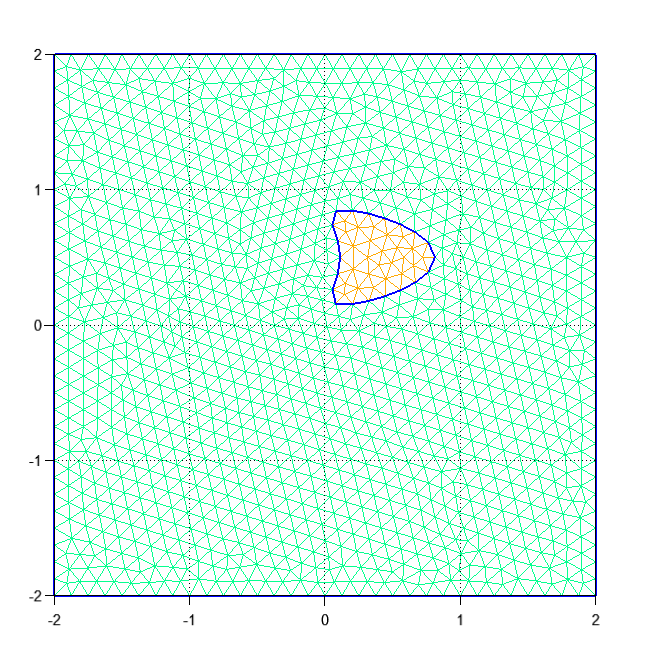
\includegraphics[width=\textwidth]{kite_sq.png}
        \caption{Kite-shaped $\Omega_1$}
    \end{subfigure}
    \begin{subfigure}{0.49\textwidth}
        \centering
        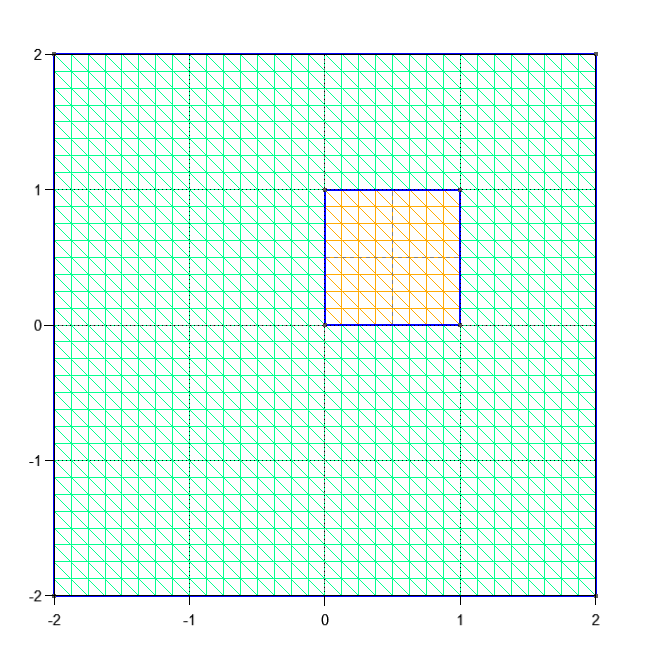
\includegraphics[width=\textwidth]{square_sq.png}
        \caption{Square-shaped $\Omega_1$}
    \end{subfigure}
    \caption{Geometries for the numerical experiments}
    \label{fig:geo}
\end{figure}

Two geometries were used in the numerical experiments
\begin{itemize}
    \item a smooth kite-shaped $\Omega_1$, given by the parametrization $\gamma:[0,2\pi]\to\mathbb{R}^2$, $t\mapsto[0.3+0.5\cos(t)+0.1625\cos(2t),0.5+0.35\sin(t)]$ and a square-shaped $\Omega\coloneqq]-2,2[\times]-2,2[.$
    \item a unit square $\Omega_1\coloneqq]0,1[^2$ inside $\Omega\coloneqq]-2,2[\times]-2,2[.$
\end{itemize}
and are illustrated in Figure~\ref{fig:geo}. $\argg(-2,y)=4,~\argg(2,y)=0,~y\in[-2,2]$ and $\eta\equiv 0$ were used as the boundary data, and $\varepsilon_1=1, \varepsilon_2=5$ were used as the permittivity of dielectrics, in both cases. The cut-off function
\begin{equation}
    w(\x)\coloneqq
    \begin{cases}
    1 & \mathrm{for}~\|\x\|< 1.4,\\
    \cos^2\left(\frac{\|\x\|-1.4}{0.5}\frac{\pi}{2}\right) & \mathrm{for}~1.4\leq\|\x\|\leq 1.9,\\
    0 & \mathrm{for}~\|\x\|> 1.9.\\
    \end{cases}
\end{equation}
was used in the volume-based formula (\ref{eq:vol-formula}).

\subsection{Results}
\begin{figure}[h!]
    \centering
    \begin{subfigure}{0.49\textwidth}
        \centering
        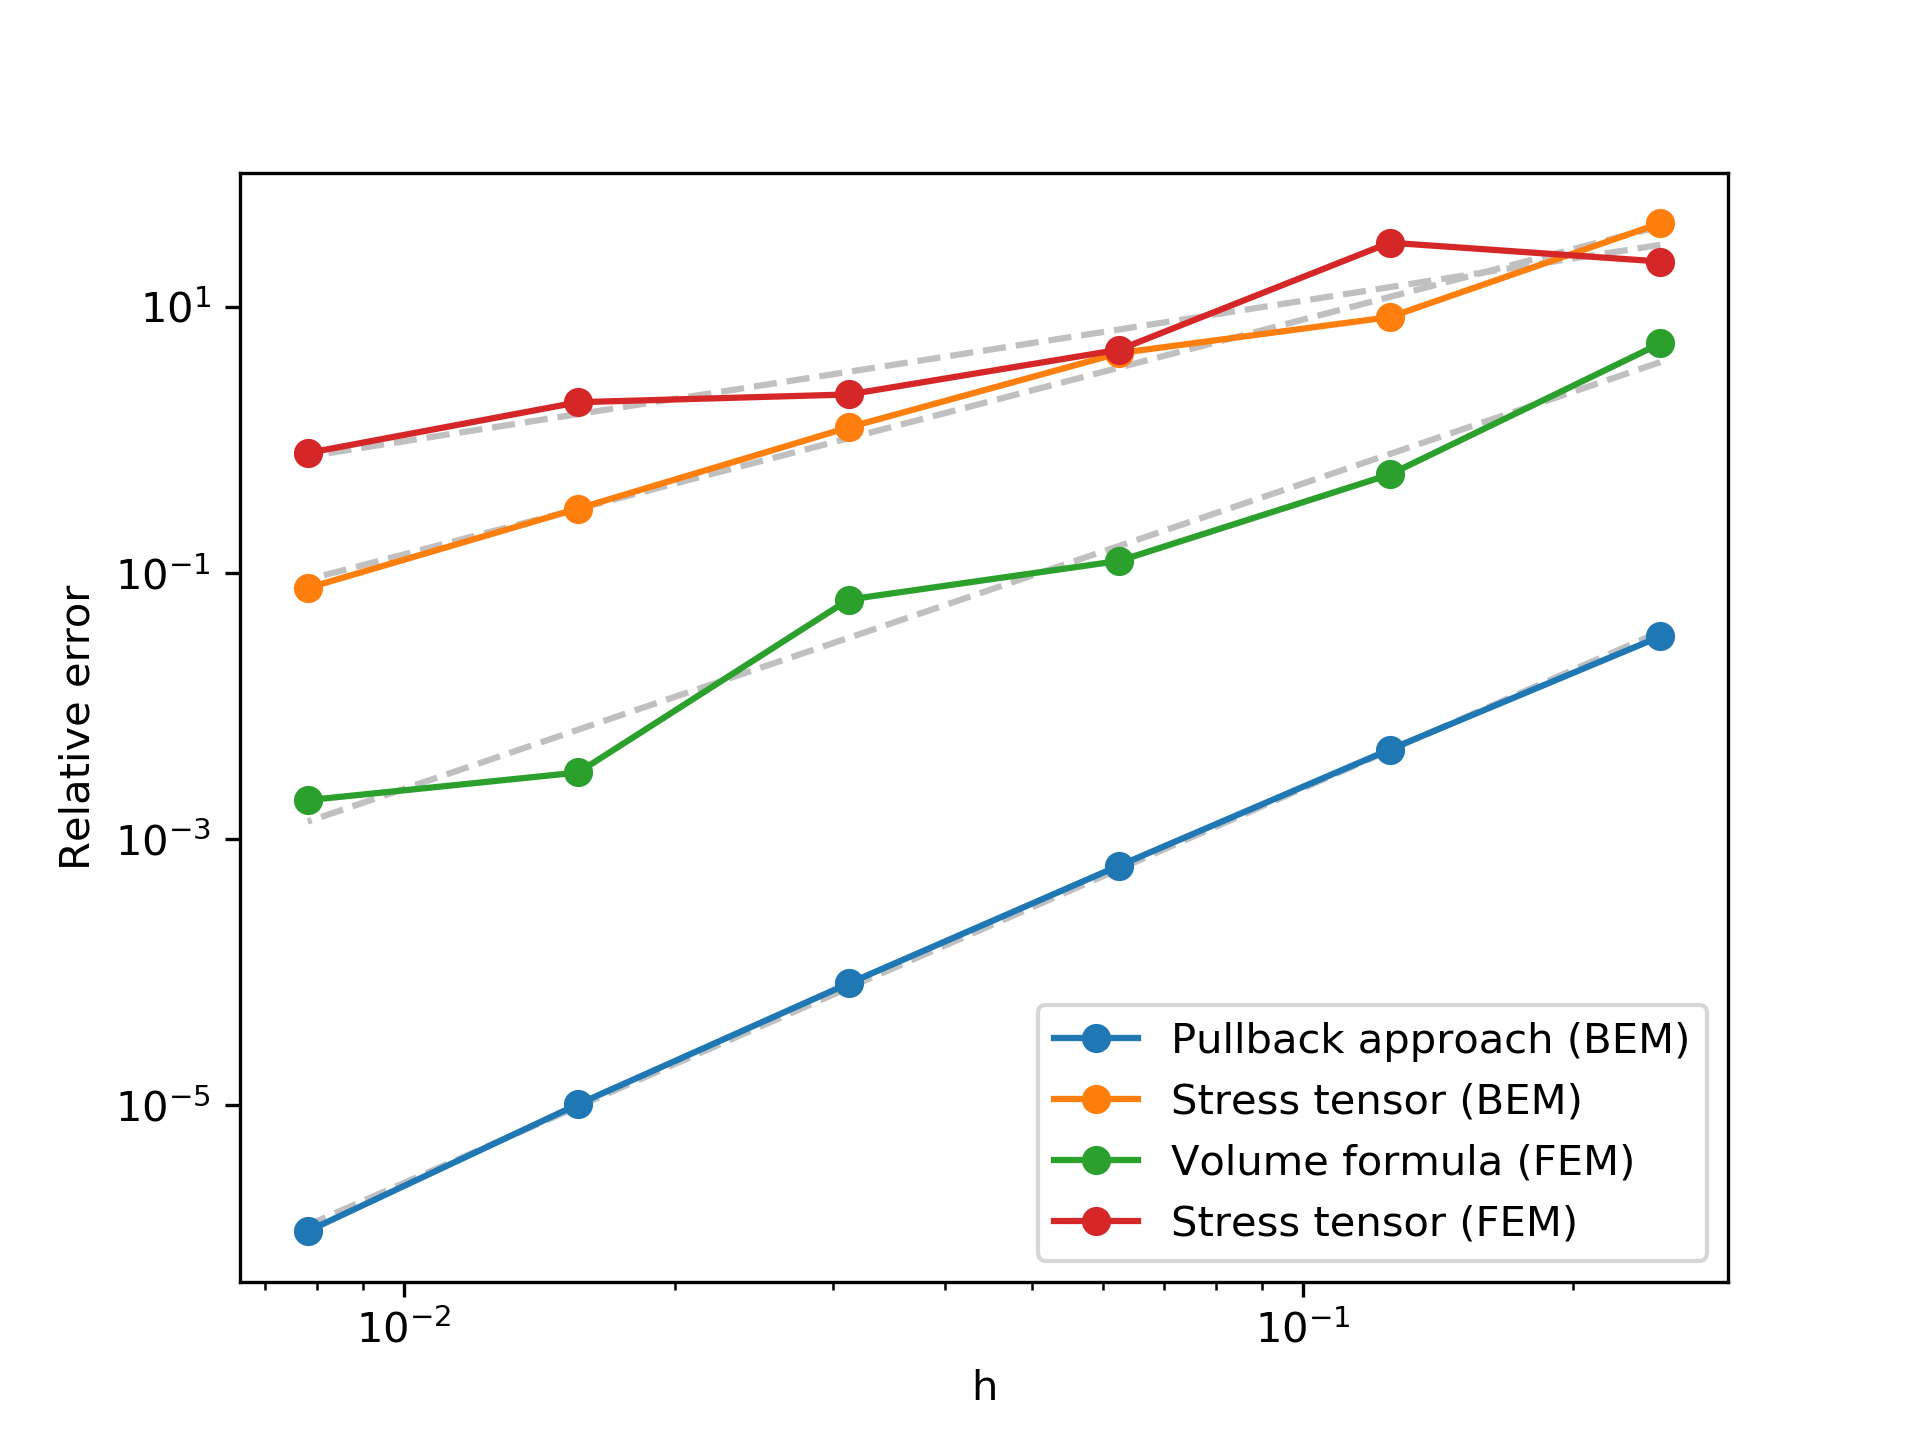
\includegraphics[width=\textwidth]{kite5_result.png}
        \caption{Kite-shaped $\Omega_1$}
    \end{subfigure}
    \begin{subfigure}{0.49\textwidth}
        \centering
        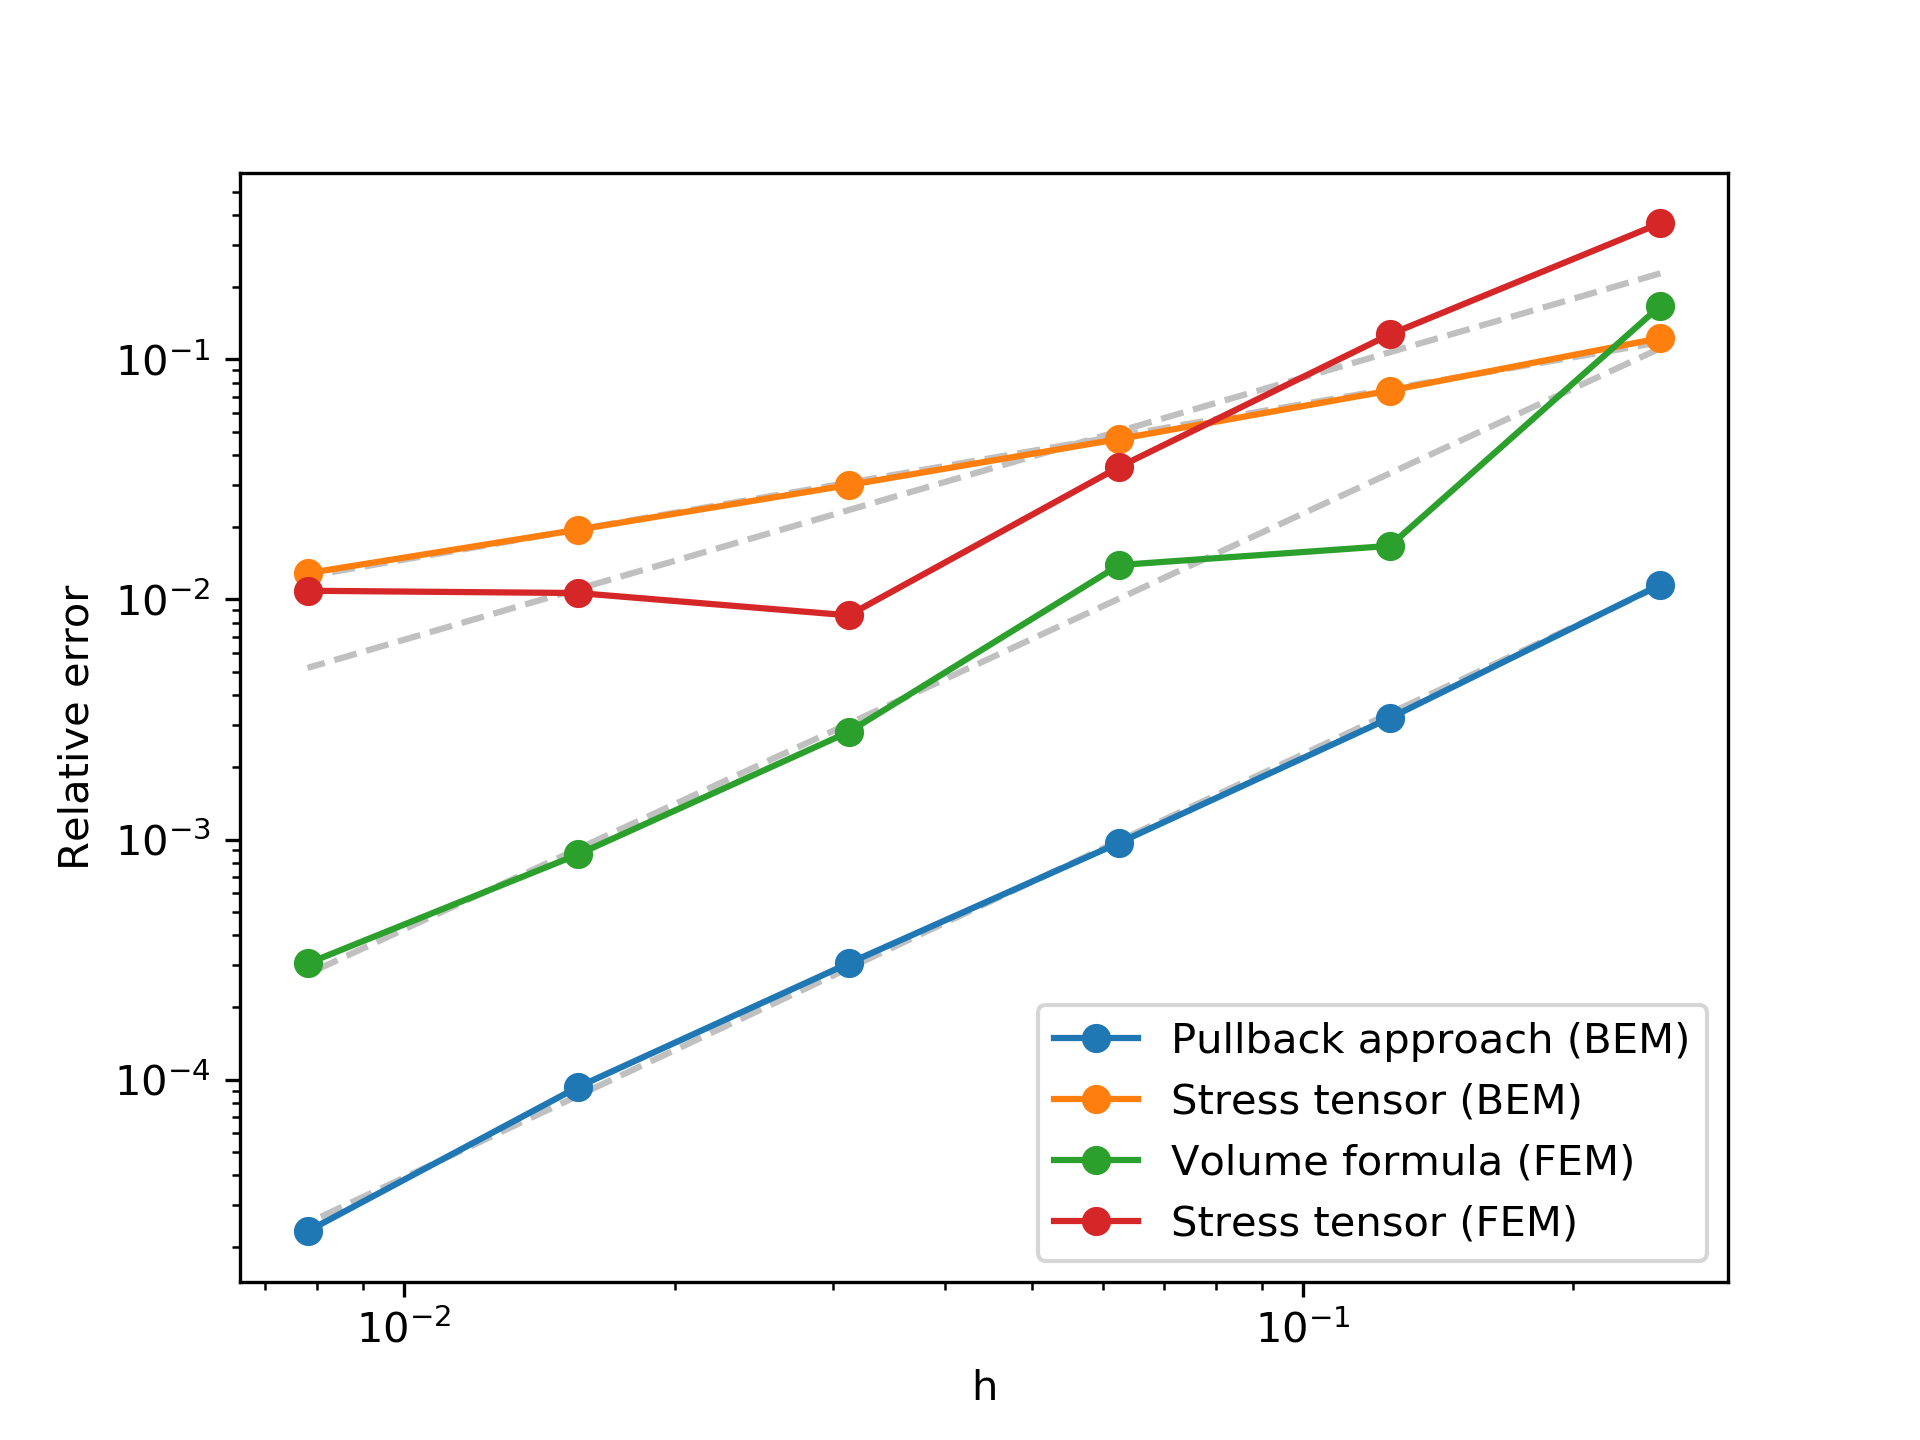
\includegraphics[width=\textwidth]{square5_result.png}
        \caption{Square-shaped $\Omega_1$}
    \end{subfigure}
    \caption{Error of total forces as a function of the meshwidth $h$. Dashed lines represent the linear regression fits.}
    \label{fig:res}
\end{figure}

 Approximations of the total force were computed according to (\ref{eq:pullback}) (``Pullback approach (BEM)") and (\ref{eq:bdry-bem}) (``Stress tensor (BEM)") using BEM, as well as (\ref{eq:vol-formula}) (``Volume formula (FEM)") and (\ref{eq:force}) (``Stress tensor (FEM)") using FEM. The Euclidean norm of the error in the computed forces is shown in Figure~\ref{fig:res} as a function of the mesh width $h$. The asymptotic rates of algebraic convergence computed by linear regression fit are listed in Table~\ref{tab:rate}. The reference solutions were computed by the pullback approach on a uniform mesh with 4728 (kite-shaped $\Omega_1$) / 5120 (square-shaped $\Omega_1$) panels.

\begin{table}[h!]
\centering
\caption{Asymptotic rate of algebraic convergence}
\begin{tabular}{|c|c|c|}
    \hline
    Method & Kite-shaped $\Omega_1$ & Square-shaped $\Omega_1$\\
    \hline
    Pullback approach (BEM) & 2.96 & 1.76 \\
    Stress tensor (BEM) & 1.76 & 0.648 \\
    Volume formula (FEM) & 2.29 & 1.73 \\
    Stress tensor (FEM) & 1.06 & 1.09 \\
    \hline
\end{tabular}
\label{tab:rate}
\end{table}

It can be observed that the pullback approach gives the best results over other methods both in terms of absolute accuracy and in terms of asymptotic rate of convergence. The performance of all methods with both smooth and non-smooth $\Omega_1$ closely match those shown in \cite{main}.

\section{Conclusion}
This work derived formulae for computation of total forces on dielectrics using shape calculus. The results demonstrated that the new approach presented in \cite{main} can be applied to transmission problems as well and outperforms classical formulae obtained from the Maxwell stress tensor. The involvement of the hypersingular operator does no harm to the fast and robust convergence of force approximation achieved by the pullback approach and brings no extra difficulty in computation.

\bibliographystyle{plain}
\bibliography{refs}

\end{document}
